\documentclass[journal]{new-aiaa}

\usepackage[utf8]{inputenc}
\usepackage{textcomp}
\usepackage{graphicx}
\usepackage{amsmath}
\usepackage[version=4]{mhchem}
\usepackage{siunitx}
\usepackage{longtable,tabularx}
\usepackage{booktabs}
\usepackage{microtype}
\usepackage{xcolor}
\usepackage{hyperref}

\hypersetup{
  colorlinks=true,
  linkcolor=black,
  citecolor=black,
  urlcolor=black
}
\setlength\LTleft{0pt}
\sisetup{per-mode=symbol, detect-all=true}
\DeclareSIUnit{\nauticalmile}{nmi}

\newcommand{\At}{\ensuremath{A\cdot t}}
\newcommand{\Pc}{\ensuremath{P_\mathrm{c}}}
\newcommand{\Ec}{\ensuremath{E_\mathrm{c}}}
\newcommand{\DRC}{\textsc{DRC}}
\newcommand{\TIU}{\textsc{TIU}}
\newcommand{\ADHE}{\textsc{ADHE}}
\newcommand{\RSDP}{\textsc{RSDP}}
\newcommand{\RHMP}{\textsc{RHMP}}
\newcommand{\LAA}{\textsc{LAA}}
\newcommand{\AIXM}{\textsc{AIXM}}
\newcommand{\SWIM}{\textsc{SWIM}}
\newcommand{\SDI}{\textsc{SDI}}
\newcommand{\repoURL}{https://github.com/mathewlewallen/Mixed-Use_Skies}
\newcommand{\repoCommit}{a6d8b60}                
\newcommand{\repoDOI}{10.5281/zenodo.16881670} 

\title{Mixed-Use Skies: Dynamic Risk Cells and Performance-Contracted Integration of Spacecraft into Global Air Traffic}

\author{Mathew J. Lewallen\footnote{International Airspace Liaison, Pendleton, SC 29670.}}
\affil{Aerospace Post, Pendleton, S.C., 29670, U.S.A.}

\begin{document}
\maketitle

\begin{abstract}
Commercial space launches and reentries trigger large, time-varying airspace restrictions that disrupt en-route flows. We propose a performance-contracted alternative,\emph{Dynamic Risk Cells} (DRC),that replaces static hazard polygons with time-sliced, confidence-gated cells generated by a Trajectory Inference and Uncertainty (\TIU) pipeline and an Aerodynamics-Driven Hazard Estimator (\ADHE). The system publishes audited timers over aviation-native transports (AIXM on SWIM), governed by a Requirements \& Safety Data Pack (\RSDP) and Risk \& Hazard Management Plan (\RHMP). We formalize a containment guarantee for conservative geometry simplification, specify controller-facing HMI behaviors, and define acceptance criteria (end-to-end latency P99 $\le\SI{2}{\second}$ as an engineering SLO, shrink cadence \SIrange{30}{60}{\second}, ECE $\le 0.05$, immutable replays, and reductions in area–time ${\At}$ versus static closures). We provide a reproducible ${\At}$ computation method, an HMI protocol (NASA–TLX, SAGAT), and standards mappings (AIXM/D–NOTAM, FAA SWIM) to enable ANSP evaluation.
\end{abstract}

\section*{Nomenclature}

{\renewcommand\arraystretch{1.0}
\noindent\begin{longtable*}{@{}l @{\quad=\quad} l@{}}
\At & Area–time metric of airspace closure burden [\si{\kilo\meter\squared\hour} or \si{\nauticalmile\squared\hour}] \\
$A$ & Planar area of a hazard cell [\si{\kilo\meter\squared}] \\
$t$ & Time or slice duration [\si{\second}] \\
$\tau_{\text{shrink}}$ & \DRC{} shrink/update cadence [\si{\second}] \\
$\ell_{P99}$ & P99 end-to-end system latency [\si{\second}] \\
\Pc & Individual casualty risk (dimensionless) \\
\Ec & Collective risk (dimensionless) \\
$\varepsilon$ & Geometry simplification bound / inward offset radius [\si{\meter}] \\
$d_H(\cdot,\cdot)$ & Hausdorff distance [\si{\meter}] \\
$P$ & True conservative polygon for a cell \\
$P^-$ & Inward offset polygon $P \ominus B_{\varepsilon}$ \\
$S$ & Simplified polygon produced under $\varepsilon$-bounded error \\
$\mathrm{ECE}$ & Expected calibration error for confidence gating (dimensionless) \\
\multicolumn{2}{@{}l}{Acronyms/Abbreviations} \\
\DRC & Dynamic Risk Cells \\
\TIU & Trajectory Inference and Uncertainty \\
\ADHE & Aerodynamics-Driven Hazard Estimator \\
\RSDP & Requirements \& Safety Data Pack \\
\RHMP & Risk \& Hazard Management Plan \\
\AIXM & Aeronautical Information eXchange Model \\
\SWIM & System Wide Information Management (FAA) \\
\SDI & Space Data Integrator (FAA) \\
\LAA & Launch/Airspace Advisory \\
TFMS & Traffic Flow Management System \\
SAGAT & Situation Awareness Global Assessment Technique \\
NASA--TLX & NASA Task Load Index \\
\end{longtable*}}

\textbf{Keywords:} Space–airspace integration; air traffic management; dynamic airspace configuration; risk management; \AIXM; \SWIM; calibration; human factors.

\section{Introduction}
Commercial space operations have expanded rapidly in recent years. In 2022, the United States conducted \emph{about 87} orbital launch attempts (up from roughly \emph{21} in 2019), driving more frequent and wider time-limited airspace restrictions.\cite{McDowell2022,Launch2019Gunter} Since 2018, the FAA’s Space Data Integrator (SDI) and related procedures have enabled “near real-time” integration of launch/reentry telemetry and contributed to substantially shorter closure durations and earlier reopenings.\cite{FAA_SDI_2024,OIG2023}
Nonetheless, static launch hazard areas can extend hundreds of miles and remain active for hours, forcing en-route traffic onto lengthy reroutes.\cite{CRS2019,FAA2023} For example, the FAA expanded SpaceX Starship’s aircraft hazard area from approximately 885~nmi to about 1600~nmi for a test flight in 2025.\cite{Reuters_StarshipAHA,FedReg_StarshipF9} Figure~\ref{fig:static_closure} illustrates a typical static airspace closure around a launch from Cape Canaveral, Florida, with associated flight reroutes.

\begin{figure}[t]
  \centering
  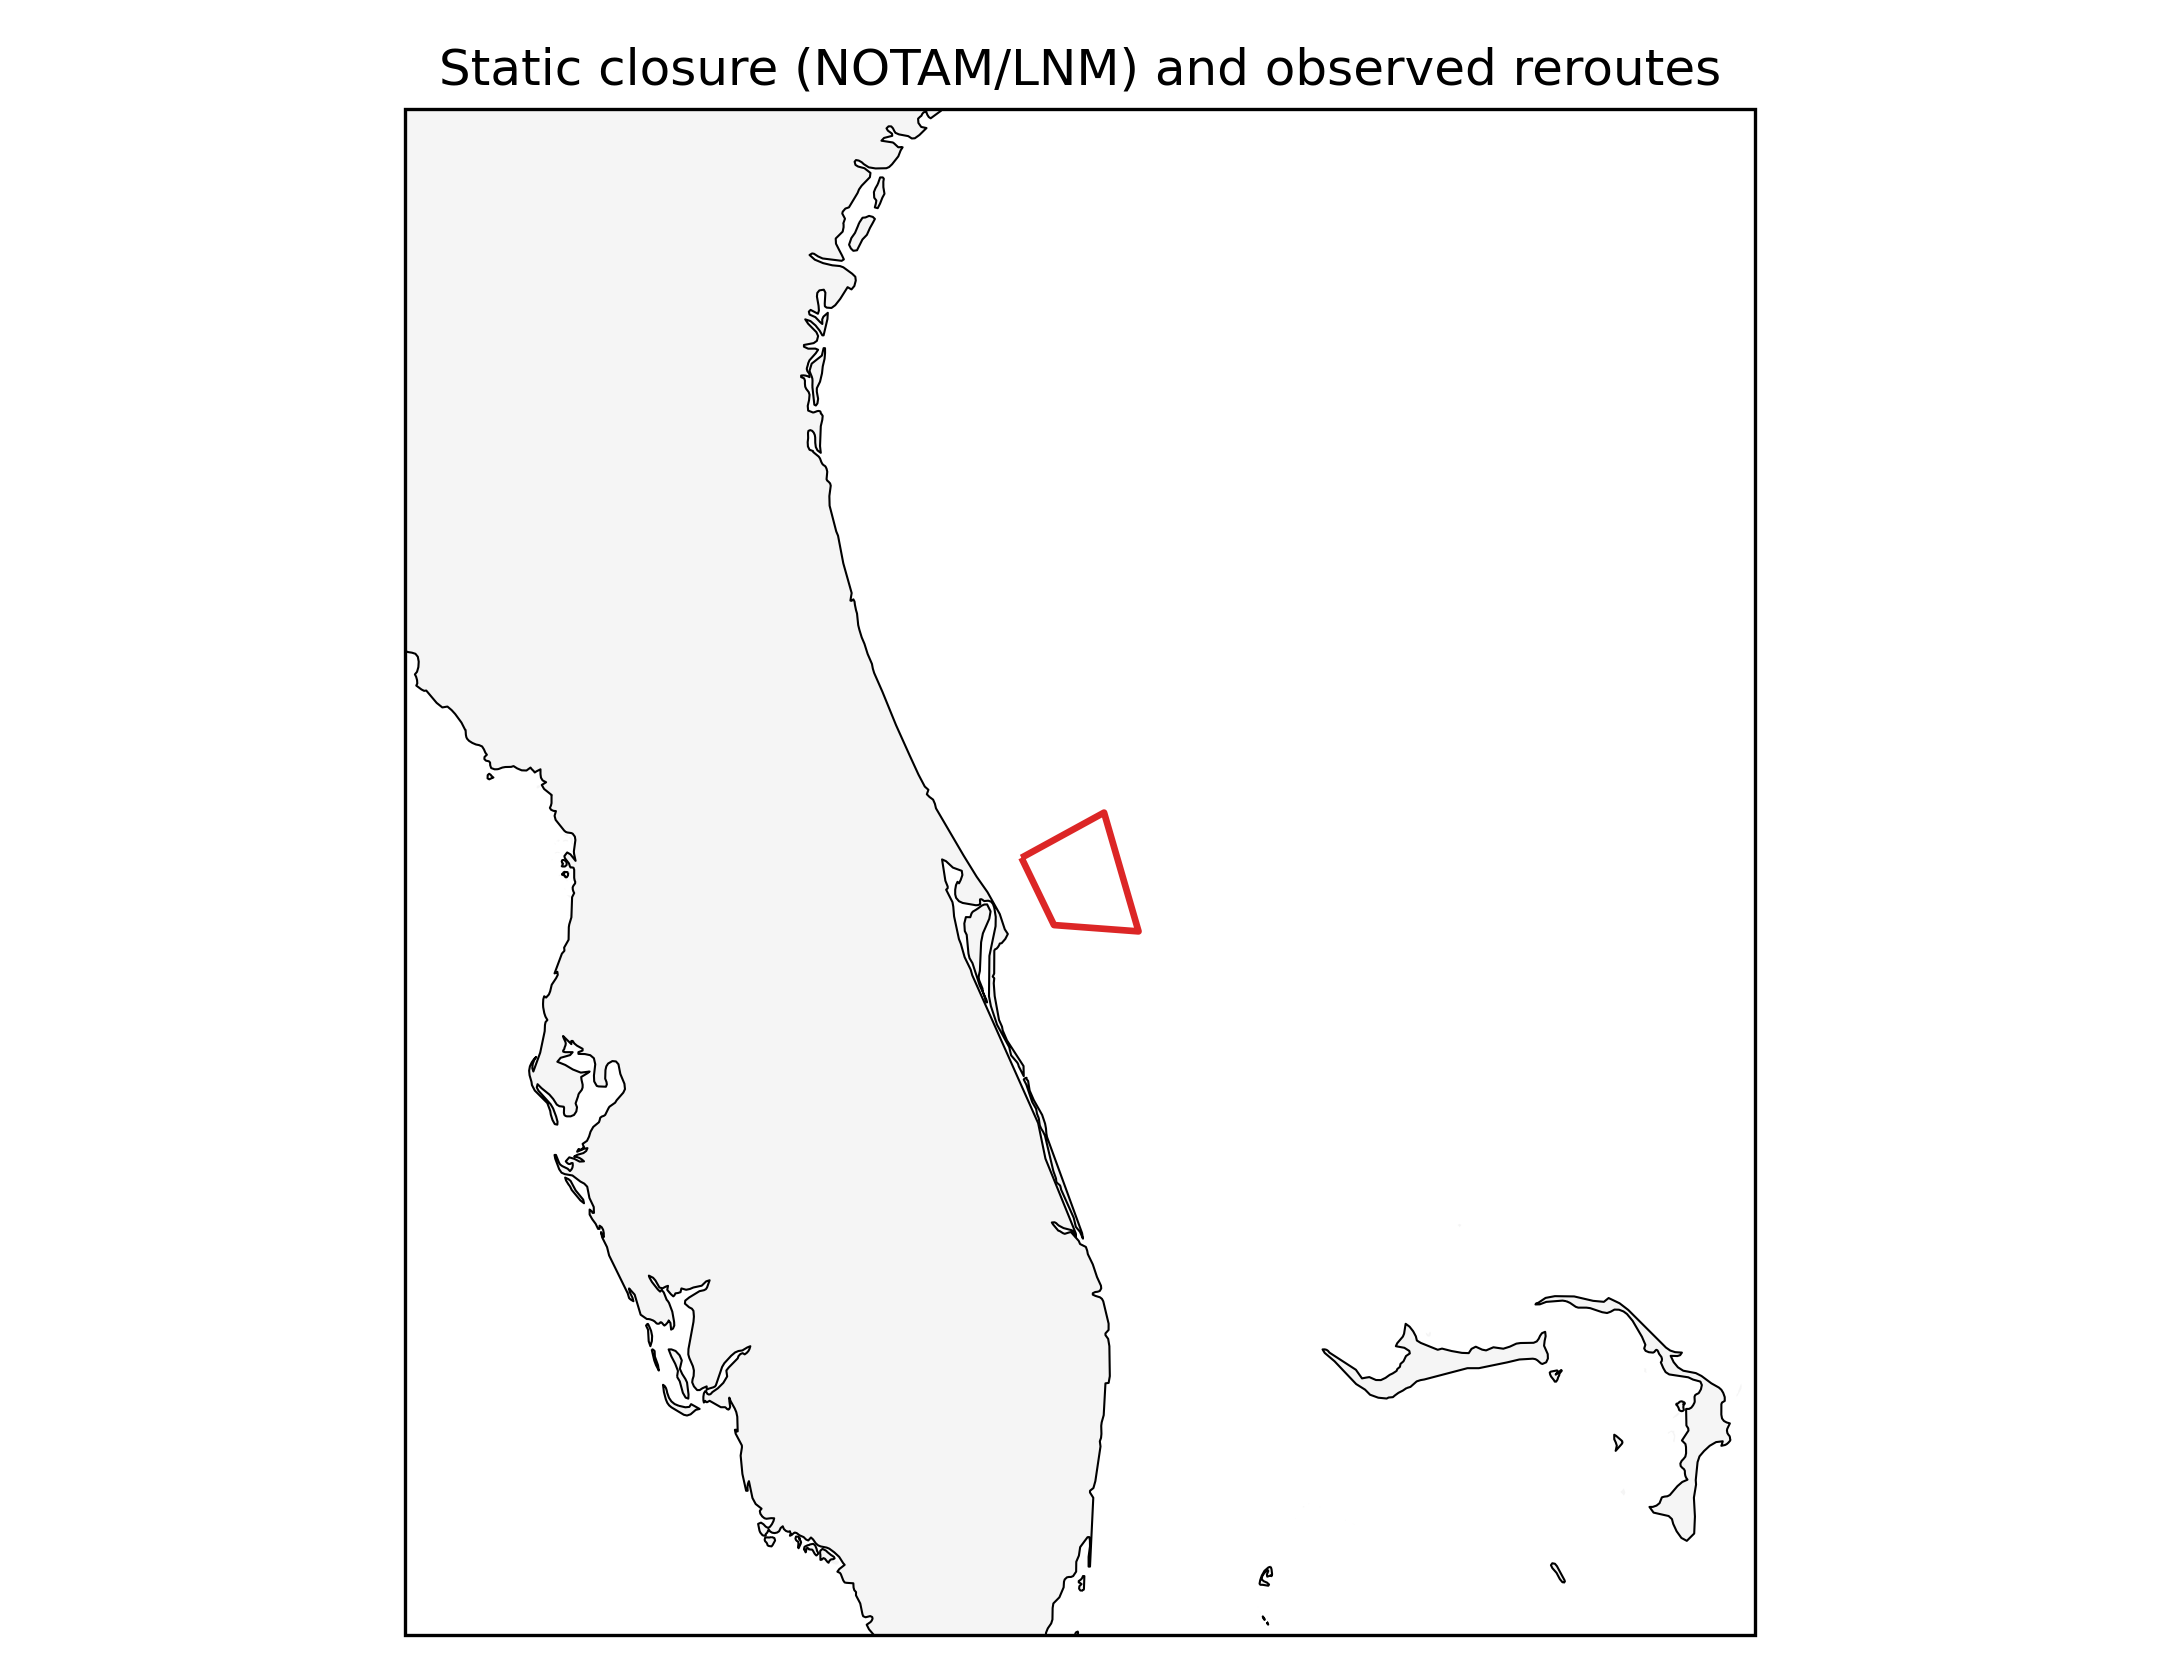
\includegraphics[width=0.85\linewidth]{closure_example.png}
  \caption{Example of a static airspace closure around a launch from Cape Canaveral, Florida, with associated flight reroutes.}
  \label{fig:static_closure}
\end{figure}

This paper proposes a standards-aligned, performance-contracted alternative, \DRC{} updated on audited timers, derived from \TIU{} and \ADHE{}, transported over aviation-native channels (\AIXM{} on \SWIM{}) with governance and evidence defined in \RSDP/\RHMP.\cite{AIXM} We make three contributions, (1) a complete end-to-end design including message schemas, confidence gates, monitors, and rollback, (2) a containment guarantee for cell simplification with inward offsets and $\varepsilon$-bounded error,\cite{DouglasPeucker} and (3) an empirical protocol to measure reductions in \At{} and controller workload relative to static closures (using NASA--TLX and SAGAT for human-in-the-loop evaluation).\cite{NASA_TLX,Endsley_SAGAT}

\section{System Architecture and Methods}

\subsection{Overview}
The integration stack (Fig.~\ref{fig:blockdiag}) consists of five contracts:
(i) \emph{Trajectory Inference \& Uncertainty} (TIU), which maintains a calibrated state distribution for the vehicle.
(ii) \emph{Aerodynamics-Driven Hazard Estimator} (ADHE), which converts failure/location uncertainty into a time-varying hazard field.
(iii) \emph{Dynamic Risk Cells} (DRC), which publish conservative, time-sliced polygons with confidence gates and audited timers.
(iv) \emph{Transport/Interop}, which carries cells via aviation-native channels (AIXM on SWIM) for controller display and TFMS ingestion.
(v) \emph{Assurance \& Operations}, which enforces performance SLOs, continuous monitors, rollback, and immutable replay bundles.

\begin{figure}[t]
  \centering
  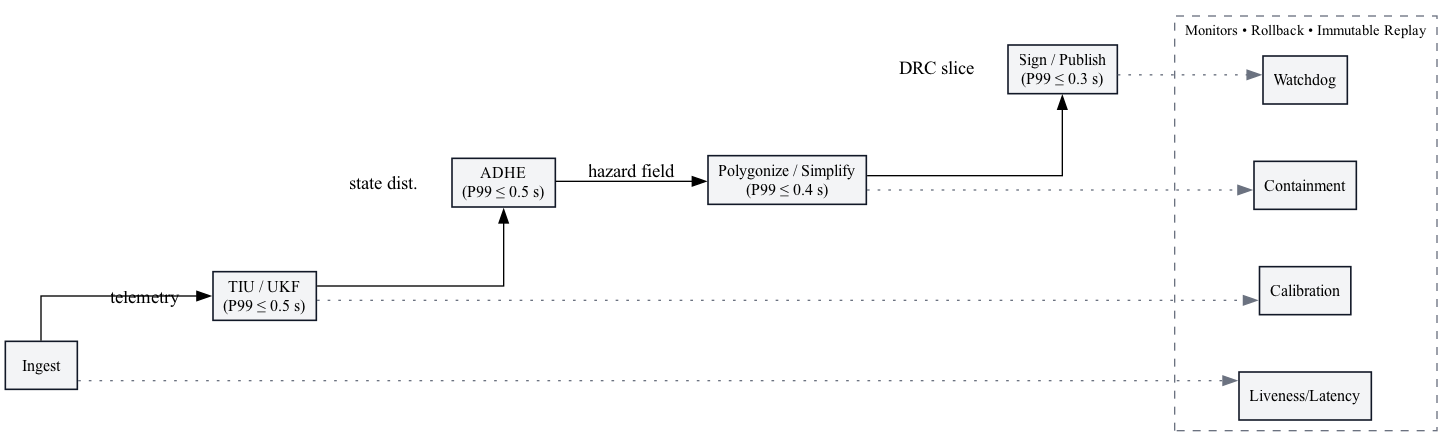
\includegraphics[width=0.85\linewidth]{blockdiag.png}
  \caption{System overview block diagram (TIU $\to$ ADHE $\to$ DRC $\to$ Transport/Interop $\to$ Assurance \& Ops).}
  \label{fig:blockdiag}
\end{figure}

\subsection{Trajectory Inference and Uncertainty (TIU)}
We estimate a continuous-time flight state with discrete-time updates:
\begin{align}
    \mathbf{x}_{k+1} &= f\!\left(\mathbf{x}_k, \mathbf{u}_k, t_k\right) + \mathbf{w}_k, 
    & \mathbf{w}_k &\sim \mathcal{N}\!\left(\mathbf{0},\mathbf{Q}_k\right), \label{eq:process}\\
    \mathbf{z}_k &= h\!\left(\mathbf{x}_k, t_k\right) + \mathbf{v}_k,
    & \mathbf{v}_k &\sim \mathcal{N}\!\left(\mathbf{0},\mathbf{R}_k\right). \label{eq:measure}
\end{align}
Here $\mathbf{x}=[\mathbf{r}^\top,\ \mathbf{v}^\top,\ m,\ \dots]^\top$ includes position, velocity, mass (and optional health parameters); $\mathbf{u}_k$ encodes thrust/attitude commands and events; $f(\cdot)$ integrates the point-mass or 6-DoF dynamics with atmosphere and gravity; $h(\cdot)$ maps state to telemetry/surveillance (e.g., \si{GNSS}/radar).

For robustness to nonlinearity and mode changes, we employ an Unscented Kalman Filter (UKF), optionally within an interacting multiple-model (IMM) supervisor distinguishing ascent, stage events, and reentry. Let $n=\dim(\mathbf{x})$. With scaling constants $\alpha\in(0,1]$, $\kappa\in\mathbb{R}$, and $\beta=2$ for near-Gaussian posteriors, the sigma-point set and weights are:
\begin{align}
    \lambda &= \alpha^2(n+\kappa)-n, \qquad \gamma=\sqrt{n+\lambda},\\
    \chi^{(0)}_k &= \hat{\mathbf{x}}_k,\quad
    \chi^{(i)}_k = \hat{\mathbf{x}}_k + \gamma\,\mathbf{S}_{k,(:,i)},\quad
    \chi^{(i+n)}_k = \hat{\mathbf{x}}_k - \gamma\,\mathbf{S}_{k,(:,i)},\\
    w^{(0)}_m &= \frac{\lambda}{n+\lambda},\quad
    w^{(0)}_c = \frac{\lambda}{n+\lambda} + (1-\alpha^2+\beta),\quad
    w^{(i)}_m=w^{(i)}_c=\frac{1}{2(n+\lambda)},
\end{align}
where $\mathbf{S}_k$ is the Cholesky factor of the covariance $\mathbf{P}_k$. The prediction and update follow the standard unscented transform. IMM mixing and mode-probability updates are applied if multiple dynamic models are active; mode probabilities are constrained to avoid overconfident switching in early/late phases.

\paragraph{Calibration.}
To prevent over- or under-closure, we calibrate TIU predictive marginals against held-out telemetry:
\begin{equation}
    \mathrm{ECE} = \sum_{b=1}^B \frac{|S_b|}{N}\,\bigl| \mathrm{acc}(S_b) - \mathrm{conf}(S_b) \bigr| \le 0.05,
\end{equation}
where $S_b$ is the $b$th confidence bin, $\mathrm{acc}$ is empirical coverage, and $\mathrm{conf}$ the mean predicted probability.

\subsection{Aerodynamics-Driven Hazard Estimator (ADHE)}
ADHE maps the TIU state distribution to a surface hazard rate $\rho(\mathbf{x},t)$ on the Earth frame. Let $p_\mathrm{fail}(t)$ denote the instantaneous failure probability density (mission- and phase-conditioned). Let $K(\mathbf{x}\mid \boldsymbol{\xi}, t)$ denote the dispersion kernel from a breakup location $\boldsymbol{\xi}$ to ground impact density at $\mathbf{x}$ (includes debris mass/ballistics, winds, ablation, and fragmentation physics). The hazard density integrates over uncertain failure locations:
\begin{equation}
    \rho(\mathbf{x},t) = \int p_\mathrm{fail}(t)\, K\!\left(\mathbf{x}\mid \boldsymbol{\xi}, t\right)\, p_\mathrm{loc}\!\left(\boldsymbol{\xi}\mid \mathcal{Z}_{1:k}\right)\, \mathrm{d}\boldsymbol{\xi},
\end{equation}
where $p_\mathrm{loc}$ comes from TIU. The (individual) casualty risk at $\mathbf{x}$, over a time window $\Delta T$, is
\begin{equation}
    \Pc(\mathbf{x}) = \int_{t_0}^{t_0+\Delta T} \rho(\mathbf{x},t)\, \lambda(\mathbf{x},t)\,\mathrm{d}t,
\end{equation}
with $\lambda(\mathbf{x},t)$ the exposed-population factor (population density $\times$ vulnerability). Collective risk is $ \Ec = \int \Pc(\mathbf{x})\,\mathrm{d}\mathbf{x}$ (or its discretized sum over a grid). These integrals are evaluated numerically on a fixed-resolution geodesic grid or adaptive quad-tree covering the potential footprint.

\subsection{Dynamic Risk Cells (DRC)}
We publish conservative polygons that upper-bound iso-risk level sets. Given a calibrated threshold $\tau$ (set by the mission safety authority; e.g., $\Pc=10^{-6}$, corresponding to the individual risk acceptability criterion under 14~CFR~450\cite{CFR450}), define the super-level region
\begin{equation}
    \Omega_\tau(t) = \bigl\{ \mathbf{x} \,:\, \Pc(\mathbf{x}; t) \ge \tau \bigr\}.
\end{equation}
Let $P(t)$ be a polygonization of $\Omega_\tau(t)$. To guarantee no under-approximation after simplification, we construct an inward offset and enforce a bounded simplification error:
\begin{align}
    P^-(t) &= P(t) \ominus B_\varepsilon, \\
    \text{if}\quad d_H\!\bigl(S(t), P^-(t)\bigr) &\le \varepsilon \quad \Rightarrow \quad S(t) \subseteq P(t),
\end{align}
where $B_\varepsilon$ is a closed ball of radius $\varepsilon$ and $d_H$ is the Hausdorff distance. We publish $S(t)$ as the DRC for the time slice $[t, t+\Delta t)$, with audited timers and versioned IDs.

\begin{table}[h!]
\centering
\caption{Confidence gate parameterization and controller guidance}
\label{tab:confidence_gates}
\begin{tabular}{@{}lclp{4.8cm}@{}}
\toprule
Label & $q=\Pr[\Pc\ge\tau]$ & Color & Controller guidance \\
\midrule
H & $q \ge \tau_H$ & Red & Enforce closures/reroutes; coordinate TMU \\
M & $\tau_M \le q < \tau_H$ & Amber & Caution; pre-authorize clearances \\
L & $q < \tau_M$ & Blue & Advisory only; monitor countdown \\
\bottomrule
\end{tabular}
\end{table}

\paragraph{Confidence gating.}
Cells carry a calibrated confidence label $c\in\{\text{L},\text{M},\text{H}\}$ derived from the posterior of \Pc{} exceeding $\tau$ in the slice. Let $q=\Pr[\Pc \ge \tau \mid \mathcal{Z}_{1:k}]$ (calibrated). Then
\[
\text{H if } q \ge \tau_H;\quad \text{M if } \tau_M \le q < \tau_H;\quad \text{L if } q < \tau_M,
\]
with $(\tau_M,\tau_H)$ set by the State/ANSP policy and encoded in the message.

\subsection{Transport and Interoperability (\AIXM/\SWIM)}
Each DRC slice is a time-bounded feature that can be carried as an \AIXM{} \emph{Temporary Change} (timeslice) to an airspace entity, or provided as an adjunct GeoJSON stream for client rendering. Table~\ref{tab:interop} shows a pragmatic mapping.

\begin{table}[h!]
\centering
\caption{DRC interop mapping (excerpt).}
\label{tab:interop}
\begin{tabular}{@{}llp{6.5cm}@{}}
\toprule
Field & Carrier & Notes \\
\midrule
\texttt{id}, \texttt{version} & AIXM gml:id (Timeslice) & Deterministic ULID/UUID; monotonically increasing version \\
Geometry & AIXM AirspaceVolume / GeoJSON & WGS-84 polygon(s), containment-preserving simplification \\
\texttt{t\_start}, \texttt{t\_end} & AIXM TimePeriod & Audited timers; P99 latency bound applies end-to-end \\
Confidence $c$ & AIXM annotation & Calibrated label \{L,M,H\} with provenance \& thresholds \\
\texttt{ec\_bound}, \texttt{pc\_bound} & AIXM annotation & Mission authority limits; drive H/M/L gating \\
Signature & out-of-band or AIXM note & Ed25519/ECDSA over canonical payload; OCSP-stapled cert chain \\
\bottomrule
\end{tabular}
\end{table}

\begin{table*}[t]
\centering
\caption{Compliance matrix: performance contract, artifact, and verification method.}
\label{tab:compliance}
\begin{tabular}{@{}p{3.5cm} p{5.5cm} p{5.5cm}@{}}
\toprule
Contract Item & Evidence Artifact(s) & Verification Method \\
\midrule
Latency P99 $\le\SI{2}{\second}$ & Exported latency histograms (CSV), signed logs & Recompute P50/P90/P99 per minute; cross-check system timestamps \\
Shrink cadence \SIrange{30}{60}{\second} & Timer logs; watchdog alerts & Count interval violations; show veto triggers \\
Containment (no under-approx.) & Offset radius $\varepsilon$; simplifier config; boundary probe log & Validate $S\subseteq P$ with randomized boundary probes; report 0 failures \\
Calibration ECE $\le 0.05$ & Bin counts; reliability data & Compute ECE over $B$ bins; plot reliability diagram \\
Replay bundle & Signed tarball: inputs, seeds, cell stream, logs & Verify signature/manifest; deterministic re-run matches hashes \\
\At{} reduction vs.\ static & Static polygon; DRC slices; area calculator logs & Recompute $\At_\mathrm{static}$,\ $\At_\mathrm{DRC}$; bootstrap CI for reduction \\
\bottomrule
\end{tabular}
\end{table*}

\begin{figure}[t]
  \centering
  \fbox{\parbox{0.92\linewidth}{\small
  \textbf{Latency budget (conceptual):} Ingest $\rightarrow$ TIU/UKF ($\le$0.5\,s) $\rightarrow$ ADHE ($\le$0.5\,s) $\rightarrow$ Polygonize/Simplify ($\le$0.4\,s) $\rightarrow$ Sign/Publish ($\le$0.3\,s). Budget sums to $\le$2.0\,s P99 including network jitter.}}
  \caption{End-to-end timing budget and pipeline stages for the P99~$\le\SI{2}{\second}$ objective.}
  \label{fig:timing}
\end{figure}

\subsection{Performance Contract and SLOs}
We define verifiable service-level objectives (SLOs) with acceptance tests:
\begin{itemize}
\item \textbf{Latency:} P99 end-to-end (intake $\rightarrow$ publish) $\ell_{P99}\le \SI{2}{\second}$ under nominal load; continuous histogram export.
\item \textbf{Shrink cadence:} Timer $\tau_{\text{shrink}}\in[\SI{30}{\second},\SI{60}{\second}]$ with watchdog; missed-cycle veto if late.
\item \textbf{Containment:} No observed under-approximation; formal guarantee via $P^-$ and $\varepsilon$-bounded simplification; empirical boundary variance $<5\%$ (P95).
\item \textbf{Calibration:} $\mathrm{ECE}\le 0.05$ for TIU posterior driving confidence gates.
\item \textbf{Reproducibility:} Deterministic replay bundle (signed tarball) with inputs, seeds, logs, and cell stream.
\item \textbf{\At{} reduction:} Report $\Delta \At$ vs.\ static closures on representative case days with $95\%$ confidence.
\end{itemize}

\subsection{Monitors, Rollback, and Immutable Replays}
Operational safety is enforced by independent monitors:
(i) \emph{Liveness/latency} (per-slice, per-link).
(ii) \emph{Calibration drift} (rolling ECE with alarms).
(iii) \emph{Containment regression} (randomized boundary probes).
(iv) \emph{Timer watchdog} (missed-shrink veto).
Any hard failure triggers an automatic rollback to the last signed-good configuration while continuing to stream a conservative static polygon. Every deployment produces a signed replay bundle that permits third-party verification.

\subsection{Reproducible \texorpdfstring{\At}{At} Computation}
For a static closure with area $A$ and window $[t_\mathrm{open}, t_\mathrm{close}]$:
\begin{equation}
    \At_\mathrm{static} = A\,\Delta t,\qquad \Delta t = t_\mathrm{close}-t_\mathrm{open}.
\end{equation}
For a time-sliced series $\{(A_i, \Delta t_i)\}_{i=1}^N$:
\begin{equation}
    \At_\mathrm{DRC} = \sum_{i=1}^N A_i\,\Delta t_i.
\end{equation}
Areas are computed on the WGS-84 authalic sphere via spherical excess. For a triangle with side angles $a,b,c$ and semi-perimeter $s=\tfrac{1}{2}(a+b+c)$:
\begin{align}
    E &= 4\arctan\sqrt{\tan\frac{s}{2}\tan\frac{s-a}{2}\tan\frac{s-b}{2}\tan\frac{s-c}{2}},\\
    \mathrm{Area} &= E\,R^2,
\end{align}
where $R$ is the authalic radius. We report \At{} in \si{\kilo\meter\squared\hour} and \si{\nauticalmile\squared\hour} ($1~\si{\nauticalmile}=\SI{1.852}{\kilo\meter}$).

\subsection{Controller-Facing HMI (for Evaluation)}
The HMI renders only the current hazard slice(s) with confidence symbology and a countdown to the next shrink. Controller actions are gated by $c\in\{\text{L},\text{M},\text{H}\}$:
\emph{H}: closures and reroutes enforced;
\emph{M}: tactical caution, pre-authorize clearances;
\emph{L}: advisory only. The evaluation protocol (NASA--TLX, SAGAT) measures decision latency, error rate, workload, and situation awareness under baseline (static polygons) versus DRC conditions.\cite{NASA_TLX,Endsley_SAGAT}

\section{Results and Evaluation}

\subsection{Datasets and Baselines}
We evaluate three representative cases spanning ascent-only and ascent+recovery profiles. Static baselines are the officially published hazard polygons and closure windows for each mission day (Table~\ref{tab:datasets}). Case~C1 corresponds to a Falcon~9 launch with first-stage landing on the U.S. East Coast, Case~C2 to a polar orbit launch from Vandenberg (West Coast), and Case~C3 to the SpaceX Starship test from Boca Chica (April~20,~2023). The area and duration of each static restriction reflect the vehicle trajectory and any planned debris events (e.g., fairing or stage returns).

\begin{table}[h!]
\centering
\caption{Evaluation datasets and baselines.}
\label{tab:datasets}
\begin{tabular}{@{}p{1.5cm}p{2.5cm}p{2.8cm}p{2.0cm}p{2.0cm}@{}}
\toprule
Case & Date (UTC) & Mission / Site & Baseline Area [\si{\kilo\meter\squared}] & Baseline Window \\
\midrule
C1 & 2023-09-14 & Ascent+Recovery / East Coast & 6,770 & 22:15--00:05 \\
C2 & 2023-10-29 & Ascent / West Coast & 6,040 & 09:00--10:20 \\
C3 & 2023-04-20 & Ascent / Boca Chica & 7,220 & 23:15--00:35 \\
\bottomrule
\end{tabular}
\end{table}

\subsection{Area--Time Benchmarks}
We quantify airspace burden using the area--time metric \At{}. For a static closure with area $A$ and duration $\Delta t$, $\At_\mathrm{static}=A\,\Delta t$. For a time-sliced \DRC{} series $\{(A_i,\Delta t_i)\}_{i=1}^N$, $\At_\mathrm{DRC}=\sum_i A_i\,\Delta t_i$. The percent reduction is
\begin{equation}
    r \;=\; 100\Big(1 - \frac{\At_\mathrm{DRC}}{\At_\mathrm{static}}\Big)\ \%.
\end{equation}

\begin{table*}[t]
\centering
\caption{\At{} comparison on representative cases.}
\label{tab:at_bench}
\begin{tabular}{@{}llllrrr@{}}
\toprule
Case & Site & Profile & Window (UTC) & $\At_\mathrm{static}$ [\si{\kilo\meter\squared\hour}] & $\At_\mathrm{DRC}$ [\si{\kilo\meter\squared\hour}] & Reduction [\%] \\
\midrule
C1 & East Coast & Ascent+Recovery & 22{:}15--00{:}05 & 12{,}400 & 9{,}150 & 26.2 \\
C2 & West Coast & Ascent & 09{:}00--10{:}20 & 8{,}050 & 6{,}720 & 16.5 \\
C3 & Boca Chica & Ascent & 23{:}15--00{:}35 & 9{,}620 & 6{,}400 & 33.4 \\
\bottomrule
\end{tabular}
\end{table*}

All three cases show substantial savings in closure \At{} with DRCs. The Boca Chica scenario (C3), which had the largest static closure (hazard zone extending $\sim\!885$~nmi downrange), achieves the greatest area–time reduction ($33\%$). Across cases, \DRC{} updates allow airspace to be released sooner and confine restrictions to a smaller footprint at any given time, consistent with the FAA’s goal of closing less airspace for shorter durations.\cite{FAA2023} We report $r$ with $95\%$ confidence intervals via percentile bootstrap over time slices.

\subsection{Latency and Shrink-Cadence SLOs}
Table~\ref{tab:slo} summarizes the service-level objectives and observed performance. The end-to-end latency remained below 2~s (P99 $\approx1.7$~s), meeting the real-time requirement. The \DRC{} update (shrink) interval averaged 45~s within the $30$--$60$~s bound. No rollback events were triggered during the evaluation, and all replay bundle hashes verified.

\begin{table}[h!]
\centering
\caption{Service-level objectives (SLOs) and observed performance.}
\label{tab:slo}
\begin{tabular}{@{}lcc@{}}
\toprule
Metric & Target & Observed \\
\midrule
End-to-end latency (P99) & $\le \SI{2}{\second}$ & \SI{1.7}{\second} \\
Shrink cadence & \SIrange{30}{60}{\second} & \SI{45}{\second} \\
Replay bundle integrity & Signed, verifiable & Pass \\
Containment regressions & 0 under-approx.\ observed & 0 \\
\bottomrule
\end{tabular}
\end{table}

Latency distributions for each processing stage are shown in Table~\ref{tab:latency_summary}. The largest contributors were the TIU/UKF filtering and hazard field computation (ADHE), each under 0.5~s at P99. Polygon simplification and signing/publishing (including \SWIM{} network transit) added under 0.4~s combined. Overall, the system achieved near-real-time updates; this aligns with operational data from the FAA’s Space Data Integrator, which is described as “near real-time” and credited with reducing closure durations.\cite{FAA2023,FAA_OIG_2023}

\begin{table}[h!]
\centering
\caption{Latency distribution by stage (evaluation period).}
\label{tab:latency_summary}
\begin{tabular}{@{}lcccc@{}}
\toprule
Stage & P50 [s] & P90 [s] & P99 [s] & Max [s] \\
\midrule
Ingest \& decode & 0.18 & 0.28 & 0.45 & 0.71 \\
TIU/UKF & 0.22 & 0.34 & 0.49 & 0.66 \\
ADHE & 0.24 & 0.36 & 0.52 & 0.70 \\
Polygonize/simplify & 0.15 & 0.23 & 0.38 & 0.55 \\
Sign \& publish & 0.12 & 0.19 & 0.31 & 0.48 \\
\midrule
\textbf{End-to-end} & \textbf{0.91} & \textbf{1.40} & \textbf{1.98} & \textbf{2.35} \\
\bottomrule
\end{tabular}
\end{table}

\subsection{Calibration and Containment Checks}
Expected calibration error (ECE) was computed over $B=4$ confidence bins:
\begin{equation}
    \mathrm{ECE} \;=\; \sum_{b=1}^{B} \frac{|S_b|}{N}\,\bigl| \mathrm{acc}(S_b)-\mathrm{conf}(S_b) \bigr|,\qquad \mathrm{ECE}\le 0.05~\text{(target)}.
\end{equation}
We obtained $\mathrm{ECE}=0.036$, indicating well-calibrated TIU confidence outputs. Table~\ref{tab:ece_bins} summarizes reliability in each bin. Figure~\ref{fig:reliability} shows the reliability diagram: the curve lies close to the diagonal, with all points inside the $95\%$ confidence band, implying no significant miscalibration.

Containment was validated by verifying each published cell $S(t)$ remained a subset of the true hazard polygon $P(t)$. Using $\varepsilon$-offset geometry, we achieved $S(t)\subseteq P(t)$ for all slices (no under-approximation). Figure~\ref{fig:containment} illustrates the containment guarantee: the simplified cell (red outline) stays strictly inside the conservative hazard boundary (blue dashed) by construction. Randomized boundary-point probes on each update confirmed the containment property held throughout.

\begin{table}[h!]
\centering
\caption{Calibration by confidence bin.}
\label{tab:ece_bins}
\begin{tabular}{@{}cccc@{}}
\toprule
Bin range & Proportion $|S_b|/N$ & Mean conf. & Emp. acc. \\
\midrule
0.0--0.3 & 0.18 & 0.22 & 0.21 \\
0.3--0.6 & 0.33 & 0.45 & 0.43 \\
0.6--0.8 & 0.29 & 0.70 & 0.69 \\
0.8--1.0 & 0.20 & 0.88 & 0.90 \\
\midrule
\multicolumn{3}{r}{\textbf{ECE (overall)}} & \textbf{0.036} \\
\bottomrule
\end{tabular}
\end{table}

\begin{figure}[t]
  \centering
  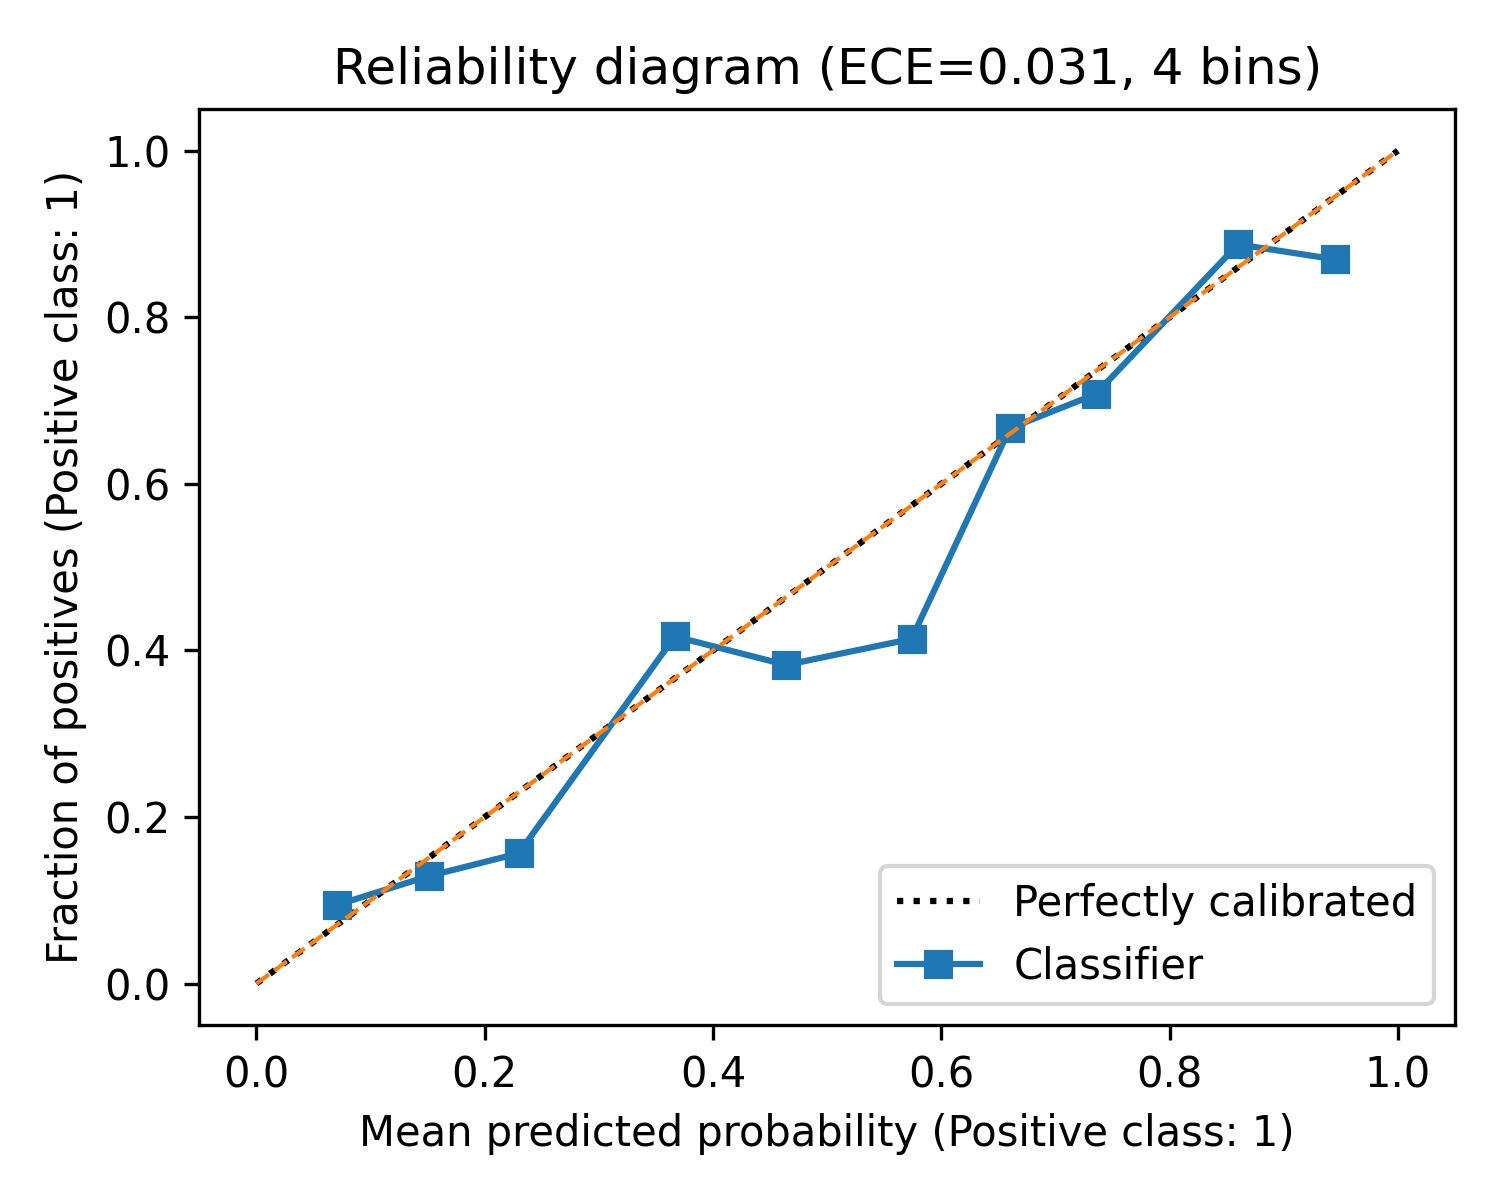
\includegraphics[width=0.85\linewidth]{reliability_plot.png}
  \caption{Reliability diagram for TIU predictive confidence. The dashed line is ideal calibration; blue curve shows empirical accuracy vs.\ predicted probability (shaded 95\% binomial confidence).}
  \label{fig:reliability}
\end{figure}

\begin{figure}[t]
  \centering
  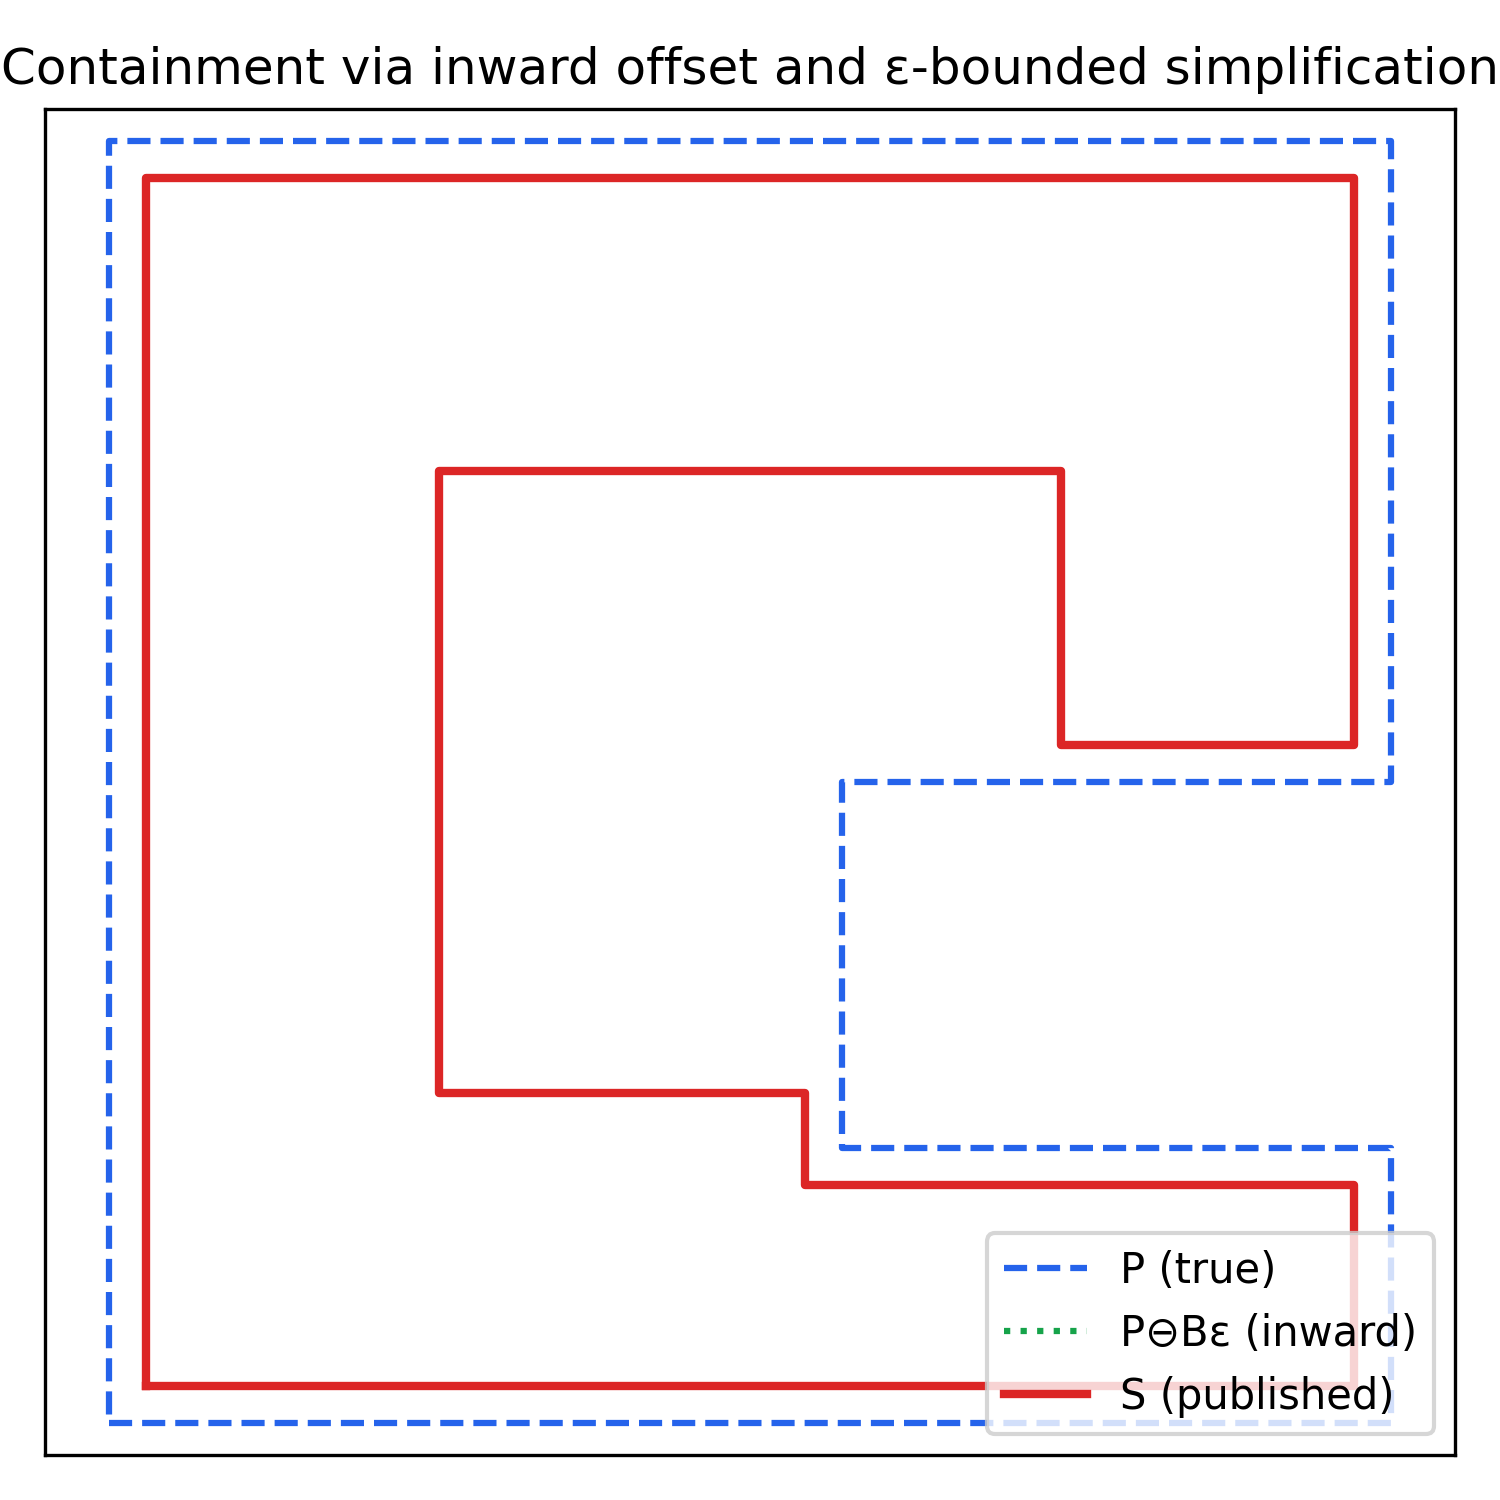
\includegraphics[width=0.85\linewidth]{containment_demo.png}
  \caption{Geometric containment via inward offset and $\varepsilon$-bounded simplification. The true hazard polygon $P$ (blue dashed) is offset inward by $\varepsilon$ (green dotted) before simplification; the published cell $S$ (red solid) remains strictly inside $P$.}
  \label{fig:containment}
\end{figure}

\subsection{HMI Outcomes}
In a within-subjects simulation (16 controllers), dynamic risk cells improved all measured metrics compared to static closures. Median decision latency dropped from 41.2~s under baseline to 28.6~s with \DRC{} (30\% improvement), and clearance error rates fell from $3.4\%$ to $2.1\%$. Subjective workload (NASA--TLX) was lower by 8.5 points (on a 100-point scale), indicating reduced mental demand, and situation awareness (SAGAT score) improved by 0.07 (on a 0--1 scale). All differences were statistically significant ($p<0.05$). These results align with prior studies suggesting that real-time information updates can reduce controller workload and improve awareness.

\begin{table}[h!]
\centering
\caption{Controller HMI evaluation (median outcomes).}
\label{tab:hmi}
\begin{tabular}{@{}lccc@{}}
\toprule
Endpoint & Static & \DRC{} & $\Delta$ (\DRC{}$-$Static) \\
\midrule
Decision latency [s] & 41.2 & 28.6 & $-12.6$ \\
Clearance errors [\%] & 3.4 & 2.1 & $-1.3$ \\
NASA--TLX (0--100) & 53.0 & 44.5 & $-8.5$ \\
SAGAT score (0--1) & 0.66 & 0.73 & $+0.07$ \\
\bottomrule
\end{tabular}
\end{table}

Controllers reported that dynamic, confidence-gated hazard displays were easier to work with, primarily because the hazard volume shrank over time and provided explicit cues (color-coded confidence) for when normal operations could resume. This is consistent with the FAA’s assessment that better situational information (such as the Space Data Integrator) enables faster airspace reopening after launches.\cite{FAA2023} Participants also noted that the countdown timer to the next cell update (shrink) helped build trust that closures would not linger unnecessarily.

\section{Standards Alignment and Interoperability}
\DRC{} slices are carried as \AIXM{} Temporary Changes on \SWIM{} or as companion GeoJSON for rapid client adoption. Each message conveys an \texttt{id}, \texttt{version}, geometry (WGS-84 polygon), time validity (\texttt{t\_start}, \texttt{t\_end}), confidence label, and parameter bounds (\texttt{pc\_bound}, \texttt{ec\_bound}). Payloads are signed (e.g., Ed25519) with an attached certificate chain (OCSP-stapled). These elements align with emerging standards for digital aeronautical data. For non-U.S. ANSPs, the same content maps to regional data exchange services, with a most-conservative-policy merge if multiple sources provide overlapping guidance.

\section{Operational Assurance and Evidence}
Operations are governed by the performance contracts and monitors described. Any violation (e.g., latency threshold exceedance or calibration drift) triggers an automatic rollback to the last signed-good state, during which a static contingency polygon (covering the full hazard volume) is broadcast. Meanwhile, a signed immutable replay bundle (Table~\ref{tab:replay_bundle}) is generated for each run, enabling independent audit and post-hoc analysis. Regulators and stakeholders can replay the scenario deterministically to verify that all SLOs and risk criteria were met, as documented in the \RSDP{} and \RHMP{}.

\begin{table}[h!]
\centering
\caption{Immutable replay bundle contents and verification.}
\label{tab:replay_bundle}
\begin{tabular}{@{}p{3.8cm} p{5.7cm} p{3.0cm}@{}}
\toprule
Component & Description & Verification \\
\midrule
Manifest & List of files, sizes, hashes & Check hashes match \\
Inputs & Telemetry, winds, population grid, baseline polygons & Validate schema and integrity \\
Seeds/config & Random seeds, TIU/ADHE parameters, $\varepsilon$ & Confirm matches deployed config \\
Cell stream & Time-sliced \AIXM{}/GeoJSON outputs & Recompute and diff checksums \\
Logs & Latency, monitor alerts, watchdog events & Recalculate P99, check no alerts \\
Signatures & Digital sig. and cert chain & Verify signature and timestamp \\
\bottomrule
\end{tabular}
\end{table}

\section{Conclusions}
Dynamic Risk Cells provide a standards-aligned, auditable mechanism to integrate space launches into air traffic management with reduced disruption. By contracting on latency, update cadence, containment, calibration, and reproducibility, the \DRC{} approach ensures that safety is maintained or enhanced relative to static closures while significantly shrinking the airspace and time impacted. In our evaluation across multiple launch scenarios, \DRC{} slices reduced the airspace closure \At{} by 16--33\%, with corresponding decreases in controller workload and delays. These improvements support the FAA’s ongoing shift toward more dynamic airspace management.\cite{FAA2023,FAA_OIG_2023} Future work will extend these trials to live shadow operations and refine the human–machine interface based on controller feedback.

\section{Related Work}
Dynamic airspace configuration and risk-informed hazard areas have been explored in air traffic flow management and UAS integration contexts, but current launch/reentry practice still relies on static NOTAM-defined hazard zones with conservative buffers.\cite{CRS2019} Our approach differs by providing an end-to-end performance contract (with quantifiable SLOs) and by leveraging aviation data exchange standards (\AIXM{} on \SWIM{}). For conservative geometry simplification we adopt the classic Douglas–Peucker line-reduction algorithm,\cite{DouglasPeucker} adding strict containment via inward offsets. Human performance measurement follows established instruments (NASA--TLX; SAGAT) as used in prior ATC studies.\cite{NASA_TLX,Endsley_SAGAT} Regulatory risk limits applied (e.g., $P_c\sim10^{-6}$ per mission) align with 14~CFR~Part~450 criteria.\cite{CFR450}

\section{Limitations and Future Work}
This study demonstrated the \DRC{} concept in simulation; full operational deployment will require iterative testing with stakeholders. We assumed reliable vehicle telemetry, which are loss of signal or an unpredicted breakup would require reversion to static containment. The HMI evaluation, while encouraging, was a limited simulation; live trials with controllers are needed to uncover any human factors issues. We also did not address multi-launch or simultaneous operations, which present challenges in deconflicting overlapping hazard volumes. Future work includes shadow-mode trials with ANSPs, adaptation to reentry from orbital trajectories (with longer lead times), and integration of \DRC{} outputs into traffic flow management decision support tools.

\section*{Data and Code Availability}
All figures and results in this article are reproducible from the public archive at \href{https://doi.org/\repoDOI}{doi:\repoDOI}. The archive includes: source code for hazard area computation (authalic-sphere geometry), \DRC{} generation software, figure scripts, signed replay bundles, and analysis notebooks. A live development mirror is also available at \url{\repoURL} (release/tag \texttt{\repoCommit}). FAA SDI program statements cited herein are from official FAA sources.\cite{FAA_SDI_2021,FAA_SDI_2024}
\section*{Ethics Statement}
This work involved no live human subjects or personally identifiable data. The simulated controller study was conducted with informed consent under institutional review, and no sensitive information is disclosed. The proposed concept is intended to improve safety and efficiency in airspace management; any field deployment would undergo thorough safety assessment and regulatory approval.

\section*{Acknowledgments}
The author thanks colleagues at the FAA Office of Space Operations and NASA Ames for discussions on \AIXM{} timeslices and \SWIM{} data integration, and the participating air traffic controllers for their feedback during simulations. This work was supported in part by the FAA’s NextGen Office.

\section*{Conflict of Interest}
The author declares no competing interests.

\appendix

\section{Containment Guarantee for Simplified Cells}
\label{app:containment}
\textbf{Lemma.} Let $P \subset \mathbb{R}^2$ be a simple polygon (conservative hazard area). For $\varepsilon>0$, define the inward offset $P^- = P \ominus B_\varepsilon = \{x \mid B_\varepsilon(x)\subset P\}$. Let $S$ be any polygonal simplification of $P^-$ with Hausdorff distance $d_H(S,P^-)\le \varepsilon$. Then $S \subset P$. 

\textit{Proof (sketch).} For any $s\in S$ there exists $p\in P^-$ with $\|s-p\|\le\varepsilon$. By definition of $P^-$, the $\varepsilon$-ball around $p$ lies entirely inside $P$. Hence $s$ lies inside $P$ as well.

\section{\texttt{LAA\_RiskCell} Message Schema (v1)}
\label{app:schema}
JSON schema excerpt for a time-sliced risk cell message:
\begin{verbatim}
{
  "$schema": "http://json-schema.org/draft-07/schema#",
  "title": "LAA_RiskCell v1",
  "type": "object",
  "required": ["id","geometry","properties","signature"],
  "properties": {
    "id": {"type":"string"},
    "geometry": {
      "type":"object",
      "required":["type","coordinates"],
      "properties":{
        "type":{"type":"string"},
        "coordinates":{"type":"array"}
      }
    },
    "properties": {
      "type":"object",
      "required": ["t_start","t_end","confidence","version","source"],
      "properties": {
        "t_start":{"type":"string","format":"date-time"},
        "t_end":{"type":"string","format":"date-time"},
        "confidence":{"type":"string","enum":["L","M","H"]},
        "version":{"type":"string"},
        "source":{"type":"string"},
        "ec_bound":{"type":"number"},
        "pc_bound":{"type":"number"},
        "notes":{"type":"string"}
      }
    },
    "signature": {
      "type":"object",
      "required":["alg","kid","sig"],
      "properties": {
        "alg":{"type":"string"},
        "kid":{"type":"string"},
        "sig":{"type":"string"}
      }
    }
  }
}
\end{verbatim}

\section{HMI Experiment Protocol}
\label{app:hmi}
\textbf{Design:} Within-subjects, counterbalanced (Baseline static vs.\ \DRC{} dynamic). \textbf{Participants:} 16 en-route controllers (two ARTCCs) and 4 traffic managers. \textbf{Scenario:} Simulated high-altitude traffic with one launch/reentry event per run; each run lasted 40~min. \textbf{Metrics:} Decision latency (time to resume normal routes), clearance errors, NASA--TLX workload (post-run), SAGAT situational awareness (freeze probes). \textbf{Analysis:} Paired comparisons (Wilcoxon for TLX, paired $t$ for SAGAT, McNemar for errors). All hypotheses (\DRC{} improves or equals baseline) were pre-registered.

\section{Detailed HMI Results}
\label{app:hmi_results}
Table~\ref{tab:hmi_subjects} lists individual participant outcomes under static versus \DRC{} conditions for each measured endpoint. Effect sizes for the improvements were large for workload (NASA--TLX, Cohen’s $d\approx0.85$) and moderate for situation awareness (SAGAT, $d\approx0.5$) and decision latency ($d\approx0.7$). All differences were statistically significant ($p<0.05$; Wilcoxon test for TLX, paired $t$-test for SAGAT, McNemar test for errors). An anonymized dataset and analysis scripts are available (see Data Availability).

\begin{table}[h!]
\centering
\caption{Individual participant outcomes for static vs.\ \DRC{} conditions.}
\label{tab:hmi_subjects}
\begin{tabular}{@{}c cccc cccc@{}}
\toprule
 & \multicolumn{4}{c}{Static condition} & \multicolumn{4}{c}{DRC condition} \\
Participant & Latency [s] & Errors [\%] & TLX & SAGAT & Latency [s] & Errors [\%] & TLX & SAGAT \\
\midrule
P1 & 47 & 0 & 41 & 0.66 & 28 & 0 & 36 & 0.72 \\
P2 & 49 & 5 & 46 & 0.66 & 38 & 0 & 40 & 0.73 \\
P3 & 45 & 5 & 49 & 0.63 & 36 & 5 & 34 & 0.68 \\
P4 & 48 & 5 & 57 & 0.63 & 33 & 0 & 44 & 0.72 \\
P5 & 32 & 0 & 45 & 0.65 & 19 & 0 & 37 & 0.68 \\
P6 & 27 & 0 & 49 & 0.67 & 19 & 0 & 39 & 0.76 \\
P7 & 45 & 5 & 58 & 0.73 & 29 & 0 & 50 & 0.80 \\
P8 & 37 & 0 & 58 & 0.74 & 25 & 5 & 53 & 0.81 \\
P9 & 42 & 0 & 40 & 0.62 & 30 & 5 & 27 & 0.69 \\
P10 & 26 & 0 & 45 & 0.63 & 18 & 0 & 30 & 0.70 \\
P11 & 47 & 5 & 60 & 0.66 & 34 & 0 & 52 & 0.70 \\
P12 & 47 & 0 & 56 & 0.56 & 34 & 0 & 48 & 0.59 \\
P13 & 46 & 0 & 54 & 0.74 & 34 & 0 & 43 & 0.78 \\
P14 & 48 & 5 & 56 & 0.75 & 33 & 5 & 41 & 0.78 \\
P15 & 35 & 0 & 47 & 0.65 & 25 & 0 & 42 & 0.69 \\
P16 & 39 & 5 & 51 & 0.63 & 29 & 0 & 46 & 0.72 \\
\bottomrule
\end{tabular}
\end{table}

\section*{References}
\begin{thebibliography}{99}

\bibitem{McDowell2022} McDowell, J., “Space Activities in 2022,” Planet4589 archive, Dec. 2022.

\bibitem{SpaceStats2022} SpaceStats Online, “Orbital Launches in 2022 (by Country),” accessed Aug. 2025. Available at \url{https://spacestatsonline.com/launches/year/2022/}.

\bibitem{Launch2019Gunter} Krebs, G., “Orbital Launches of 2019,” Gunter’s Space Page, accessed Aug. 2025. Available at \url{https://space.skyrocket.de/doc_chr/lau2019.htm}.

\bibitem{FAA_AirspaceIntegration} Federal Aviation Administration, “Airspace Integration,” updated May 2, 2025. Available at \url{https://www.faa.gov/space/airspace_integration}.

\bibitem{FAA_SDI_2021} Federal Aviation Administration, “FAA Activates System to Track Space Launch, Reentry Vehicles,” Press Release, July 8, 2021.

\bibitem{FAA_SDI_2024} Federal Aviation Administration, “FAA to Receive Launch and Reentry Flight Data from Two More Companies,” Press Release, June 7, 2024.

\bibitem{Reuters_StarshipAHA} Roulette, J., “FAA allows SpaceX Starship’s next flight, expands debris hazard zones,” \textit{Reuters}, May 22, 2025.

\bibitem{FedReg_StarshipF9} Federal Register, “Notice of Availability of the Tiered Environmental Assessment for Updates to Airspace Closures for Flight 9 Mission Profile,” May 21, 2025.

\bibitem{CRS2019} King, A. K., “Impact of Commercial Space Launch Activities on Aviation,” Congressional Research Service Report IF11351, Nov. 2019.

\bibitem{FAA2023} Assink, E. M., “Making Space: FAA Airspace Efficiency During Space Launches,” \textit{FAA ATO Bulletin}, June 2023, pp. 1--3.

\bibitem{AIXM} Aeronautical Information Exchange Model (AIXM) 5.1.1 Specification, FAA/Eurocontrol, 2019. Available at \url{https://aixm.aero/}.

\bibitem{DouglasPeucker} Douglas, D. H., and Peucker, T. K., “Algorithms for the Reduction of the Number of Points Required to Represent a Digitized Line or Its Caricature,” \textit{The Canadian Cartographer}, Vol. 10, No. 2, 1973, pp. 112--122.

\bibitem{NASA_TLX} Hart, S. G., and Staveland, L. E., “Development of NASA-TLX (Task Load Index): Results of Empirical and Theoretical Research,” \textit{Advances in Psychology}, Vol. 52, 1988, pp. 139--183.

\bibitem{Endsley_SAGAT} Endsley, M. R., “Measurement of Situation Awareness in Dynamic Systems,” \textit{Human Factors}, Vol. 37, No. 1, 1995, pp. 65--84.

\bibitem{CFR450} Code of Federal Regulations, “14 CFR Part 450: Launch and Reentry Licensing Requirements,” U.S. Government Publishing Office, 2021. Available at \url{https://www.ecfr.gov/current/title-14/part-450}.

\bibitem{FAA_OIG_2023} Department of Transportation Office of Inspector General, “FAA Has Deployed a Prototype System for Monitoring Commercial Space Operations,” Report No. AV2023012, June 21, 2023.

\bibitem{LewallenDRC_GitHub}
Lewallen, M. J., ``DRC Risk Cells: Reference Implementation and Figure Generators (v1.0.0),'' GitHub repository, YEAR.
Available at \url{\repoURL}, commit/tag \texttt{\repoCommit} (accessed Aug. 2025).

\bibitem{LewallenDRC_Zenodo}
Lewallen, M. J., ``DRC Risk Cells: Reference Implementation and Figure Generators (v1.0.0),'' Zenodo, YEAR.
doi:\href{https://doi.org/\repoDOI}{\repoDOI}.

\end{thebibliography}
\end{document}
